\gdef\sfill{white}
\gdef\Afill{white}
\gdef\Bfill{white}
\gdef\Cfill{white}
\gdef\Dfill{white}
\gdef\Efill{white}
\gdef\Ffill{white}
\gdef\Gfill{white}

\gdef\sdesc{s}
\gdef\Adesc{A}
\gdef\Bdesc{B}
\gdef\Cdesc{C}
\gdef\Ddesc{D}
\gdef\Edesc{E}
\gdef\Fdesc{F}
\gdef\Gdesc{G}
\gdef\sdesc{s[/]}
\gdef\Adesc{A[/]}
\gdef\Bdesc{B[/]}
\gdef\Cdesc{C[/]}
\gdef\Ddesc{D[/]}
\gdef\Edesc{E[/]}
\gdef\Fdesc{F[/]}
\gdef\Gdesc{G[/]}

\begin{tabular}{c}
Graph\\
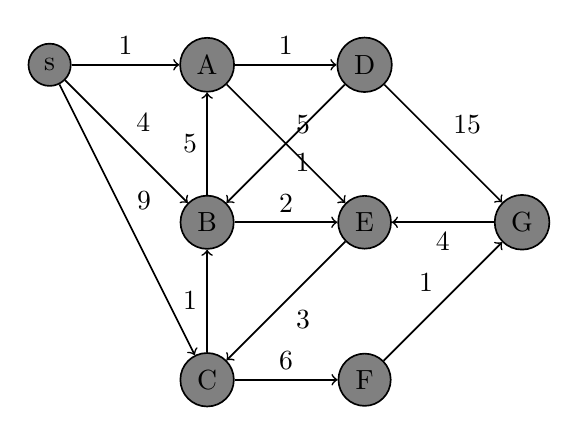
\begin{tikzpicture}[->, semithick,auto, node distance=2cm]


\node[draw, circle, fill=\sfill] (s) at (0,0) {s};
\node[draw, circle, fill=\Afill] (A) [right of=s] {A};
\node[draw, circle, fill=\Bfill] (B) [below of=A] {B};
\node[draw, circle, fill=\Cfill] (C) [below of=B] {C};
\node[draw, circle, fill=\Dfill] (D) [right of=A] {D};
\node[draw, circle, fill=\Efill] (E) [below of=D] {E};
\node[draw, circle, fill=\Ffill] (F) [below of=E] {F};
\node[draw, circle, fill=\Gfill] (G) [right of=E] {G};

\path 	(s) 	edge node {1} (A)
		edge node {4} (B)
		edge node {9} (C)
	(A) 	edge node {1} (D)
		edge node {5} (E)
	(B) 	edge node {5} (A)
		edge node {2} (E)
	(C) 	edge node {1} (B)
		edge node {6} (F)
	(D) 	edge node {1} (B)
		edge node {15} (G)
	(E) 	edge node {3} (C)
	(F) 	edge node {1} (G)
	(G) 	edge node {4} (E)
	;

\end{tikzpicture}

\\
\gdef\sfill{gray}
\gdef\sdesc{s[1/]}
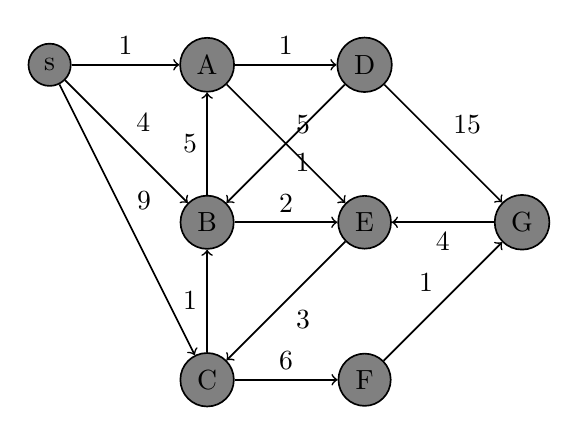
\begin{tikzpicture}[->, semithick,auto, node distance=2cm]


\node[draw, circle, fill=\sfill] (s) at (0,0) {s};
\node[draw, circle, fill=\Afill] (A) [right of=s] {A};
\node[draw, circle, fill=\Bfill] (B) [below of=A] {B};
\node[draw, circle, fill=\Cfill] (C) [below of=B] {C};
\node[draw, circle, fill=\Dfill] (D) [right of=A] {D};
\node[draw, circle, fill=\Efill] (E) [below of=D] {E};
\node[draw, circle, fill=\Ffill] (F) [below of=E] {F};
\node[draw, circle, fill=\Gfill] (G) [right of=E] {G};

\path 	(s) 	edge node {1} (A)
		edge node {4} (B)
		edge node {9} (C)
	(A) 	edge node {1} (D)
		edge node {5} (E)
	(B) 	edge node {5} (A)
		edge node {2} (E)
	(C) 	edge node {1} (B)
		edge node {6} (F)
	(D) 	edge node {1} (B)
		edge node {15} (G)
	(E) 	edge node {3} (C)
	(F) 	edge node {1} (G)
	(G) 	edge node {4} (E)
	;

\end{tikzpicture}

\\
\gdef\Afill{gray}
\gdef\Adesc{A[2/]}
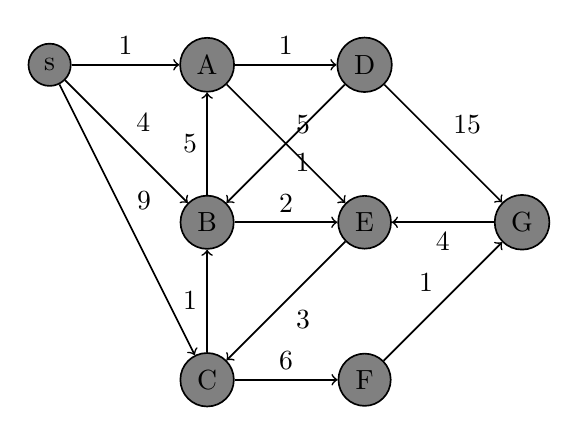
\begin{tikzpicture}[->, semithick,auto, node distance=2cm]


\node[draw, circle, fill=\sfill] (s) at (0,0) {s};
\node[draw, circle, fill=\Afill] (A) [right of=s] {A};
\node[draw, circle, fill=\Bfill] (B) [below of=A] {B};
\node[draw, circle, fill=\Cfill] (C) [below of=B] {C};
\node[draw, circle, fill=\Dfill] (D) [right of=A] {D};
\node[draw, circle, fill=\Efill] (E) [below of=D] {E};
\node[draw, circle, fill=\Ffill] (F) [below of=E] {F};
\node[draw, circle, fill=\Gfill] (G) [right of=E] {G};

\path 	(s) 	edge node {1} (A)
		edge node {4} (B)
		edge node {9} (C)
	(A) 	edge node {1} (D)
		edge node {5} (E)
	(B) 	edge node {5} (A)
		edge node {2} (E)
	(C) 	edge node {1} (B)
		edge node {6} (F)
	(D) 	edge node {1} (B)
		edge node {15} (G)
	(E) 	edge node {3} (C)
	(F) 	edge node {1} (G)
	(G) 	edge node {4} (E)
	;

\end{tikzpicture}

\\
\gdef\Dfill{gray}
\gdef\Ddesc{D[3/]}
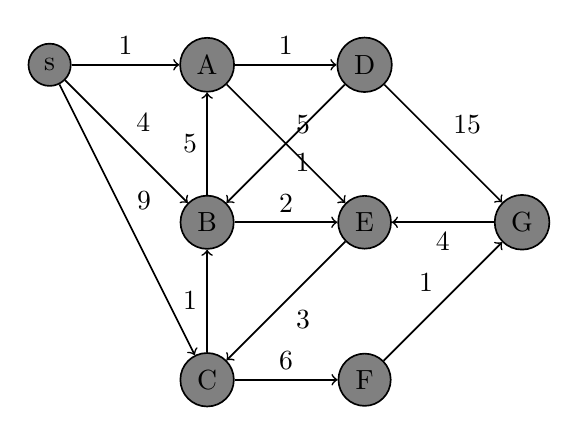
\begin{tikzpicture}[->, semithick,auto, node distance=2cm]


\node[draw, circle, fill=\sfill] (s) at (0,0) {s};
\node[draw, circle, fill=\Afill] (A) [right of=s] {A};
\node[draw, circle, fill=\Bfill] (B) [below of=A] {B};
\node[draw, circle, fill=\Cfill] (C) [below of=B] {C};
\node[draw, circle, fill=\Dfill] (D) [right of=A] {D};
\node[draw, circle, fill=\Efill] (E) [below of=D] {E};
\node[draw, circle, fill=\Ffill] (F) [below of=E] {F};
\node[draw, circle, fill=\Gfill] (G) [right of=E] {G};

\path 	(s) 	edge node {1} (A)
		edge node {4} (B)
		edge node {9} (C)
	(A) 	edge node {1} (D)
		edge node {5} (E)
	(B) 	edge node {5} (A)
		edge node {2} (E)
	(C) 	edge node {1} (B)
		edge node {6} (F)
	(D) 	edge node {1} (B)
		edge node {15} (G)
	(E) 	edge node {3} (C)
	(F) 	edge node {1} (G)
	(G) 	edge node {4} (E)
	;

\end{tikzpicture}

\\
\gdef\Bfill{gray}
\gdef\Bdesc{B[4/]}
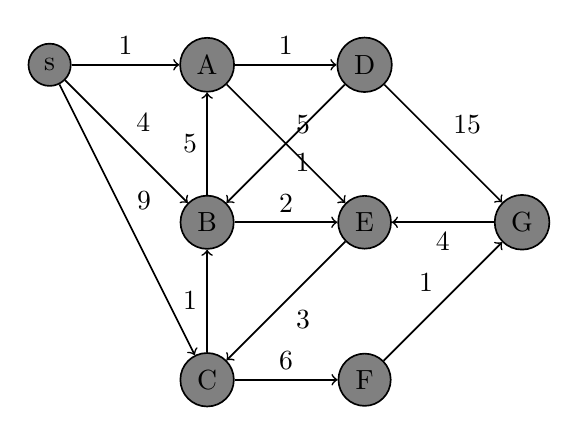
\begin{tikzpicture}[->, semithick,auto, node distance=2cm]


\node[draw, circle, fill=\sfill] (s) at (0,0) {s};
\node[draw, circle, fill=\Afill] (A) [right of=s] {A};
\node[draw, circle, fill=\Bfill] (B) [below of=A] {B};
\node[draw, circle, fill=\Cfill] (C) [below of=B] {C};
\node[draw, circle, fill=\Dfill] (D) [right of=A] {D};
\node[draw, circle, fill=\Efill] (E) [below of=D] {E};
\node[draw, circle, fill=\Ffill] (F) [below of=E] {F};
\node[draw, circle, fill=\Gfill] (G) [right of=E] {G};

\path 	(s) 	edge node {1} (A)
		edge node {4} (B)
		edge node {9} (C)
	(A) 	edge node {1} (D)
		edge node {5} (E)
	(B) 	edge node {5} (A)
		edge node {2} (E)
	(C) 	edge node {1} (B)
		edge node {6} (F)
	(D) 	edge node {1} (B)
		edge node {15} (G)
	(E) 	edge node {3} (C)
	(F) 	edge node {1} (G)
	(G) 	edge node {4} (E)
	;

\end{tikzpicture}

\\
\gdef\Efill{gray}
\gdef\Edesc{E[5/]}
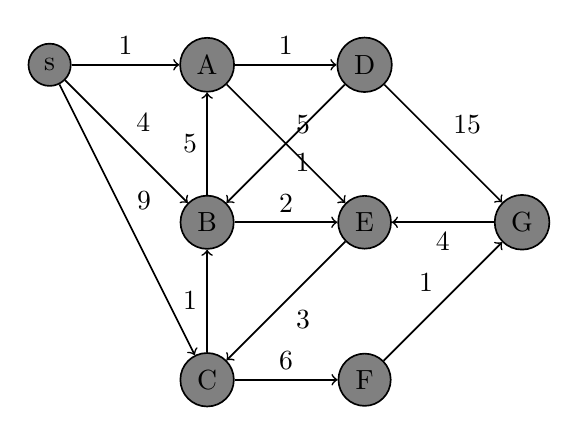
\begin{tikzpicture}[->, semithick,auto, node distance=2cm]


\node[draw, circle, fill=\sfill] (s) at (0,0) {s};
\node[draw, circle, fill=\Afill] (A) [right of=s] {A};
\node[draw, circle, fill=\Bfill] (B) [below of=A] {B};
\node[draw, circle, fill=\Cfill] (C) [below of=B] {C};
\node[draw, circle, fill=\Dfill] (D) [right of=A] {D};
\node[draw, circle, fill=\Efill] (E) [below of=D] {E};
\node[draw, circle, fill=\Ffill] (F) [below of=E] {F};
\node[draw, circle, fill=\Gfill] (G) [right of=E] {G};

\path 	(s) 	edge node {1} (A)
		edge node {4} (B)
		edge node {9} (C)
	(A) 	edge node {1} (D)
		edge node {5} (E)
	(B) 	edge node {5} (A)
		edge node {2} (E)
	(C) 	edge node {1} (B)
		edge node {6} (F)
	(D) 	edge node {1} (B)
		edge node {15} (G)
	(E) 	edge node {3} (C)
	(F) 	edge node {1} (G)
	(G) 	edge node {4} (E)
	;

\end{tikzpicture}

\\
\gdef\Cfill{gray}
\gdef\Cdesc{s[6/]}
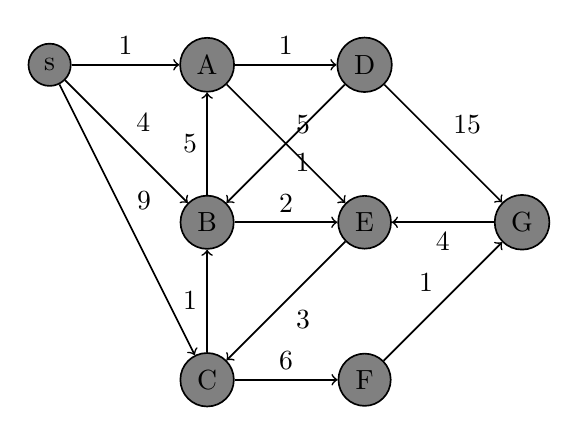
\begin{tikzpicture}[->, semithick,auto, node distance=2cm]


\node[draw, circle, fill=\sfill] (s) at (0,0) {s};
\node[draw, circle, fill=\Afill] (A) [right of=s] {A};
\node[draw, circle, fill=\Bfill] (B) [below of=A] {B};
\node[draw, circle, fill=\Cfill] (C) [below of=B] {C};
\node[draw, circle, fill=\Dfill] (D) [right of=A] {D};
\node[draw, circle, fill=\Efill] (E) [below of=D] {E};
\node[draw, circle, fill=\Ffill] (F) [below of=E] {F};
\node[draw, circle, fill=\Gfill] (G) [right of=E] {G};

\path 	(s) 	edge node {1} (A)
		edge node {4} (B)
		edge node {9} (C)
	(A) 	edge node {1} (D)
		edge node {5} (E)
	(B) 	edge node {5} (A)
		edge node {2} (E)
	(C) 	edge node {1} (B)
		edge node {6} (F)
	(D) 	edge node {1} (B)
		edge node {15} (G)
	(E) 	edge node {3} (C)
	(F) 	edge node {1} (G)
	(G) 	edge node {4} (E)
	;

\end{tikzpicture}

\\
\gdef\Ffill{gray}
\gdef\Fdesc{F[7/]}
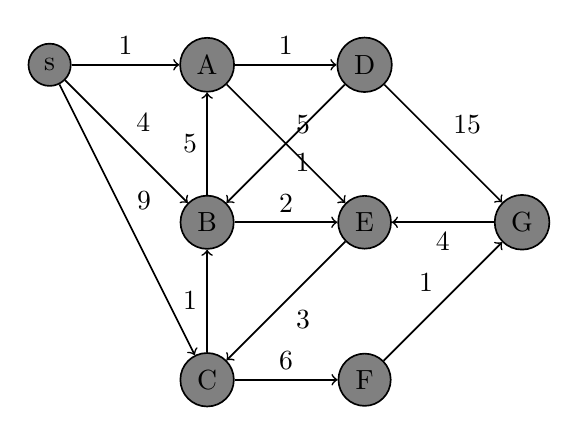
\begin{tikzpicture}[->, semithick,auto, node distance=2cm]


\node[draw, circle, fill=\sfill] (s) at (0,0) {s};
\node[draw, circle, fill=\Afill] (A) [right of=s] {A};
\node[draw, circle, fill=\Bfill] (B) [below of=A] {B};
\node[draw, circle, fill=\Cfill] (C) [below of=B] {C};
\node[draw, circle, fill=\Dfill] (D) [right of=A] {D};
\node[draw, circle, fill=\Efill] (E) [below of=D] {E};
\node[draw, circle, fill=\Ffill] (F) [below of=E] {F};
\node[draw, circle, fill=\Gfill] (G) [right of=E] {G};

\path 	(s) 	edge node {1} (A)
		edge node {4} (B)
		edge node {9} (C)
	(A) 	edge node {1} (D)
		edge node {5} (E)
	(B) 	edge node {5} (A)
		edge node {2} (E)
	(C) 	edge node {1} (B)
		edge node {6} (F)
	(D) 	edge node {1} (B)
		edge node {15} (G)
	(E) 	edge node {3} (C)
	(F) 	edge node {1} (G)
	(G) 	edge node {4} (E)
	;

\end{tikzpicture}

\\
\gdef\Gfill{gray}
\gdef\Gdesc{G[8/]}
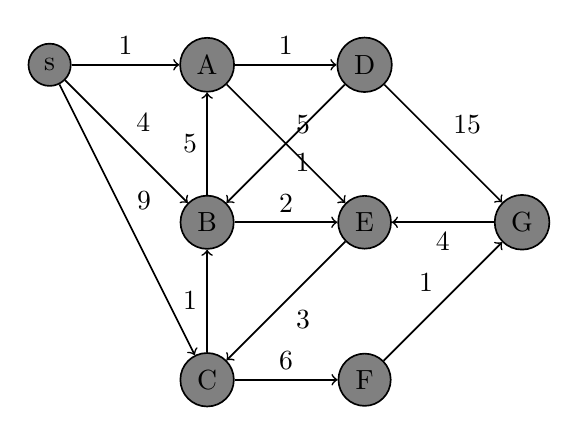
\begin{tikzpicture}[->, semithick,auto, node distance=2cm]


\node[draw, circle, fill=\sfill] (s) at (0,0) {s};
\node[draw, circle, fill=\Afill] (A) [right of=s] {A};
\node[draw, circle, fill=\Bfill] (B) [below of=A] {B};
\node[draw, circle, fill=\Cfill] (C) [below of=B] {C};
\node[draw, circle, fill=\Dfill] (D) [right of=A] {D};
\node[draw, circle, fill=\Efill] (E) [below of=D] {E};
\node[draw, circle, fill=\Ffill] (F) [below of=E] {F};
\node[draw, circle, fill=\Gfill] (G) [right of=E] {G};

\path 	(s) 	edge node {1} (A)
		edge node {4} (B)
		edge node {9} (C)
	(A) 	edge node {1} (D)
		edge node {5} (E)
	(B) 	edge node {5} (A)
		edge node {2} (E)
	(C) 	edge node {1} (B)
		edge node {6} (F)
	(D) 	edge node {1} (B)
		edge node {15} (G)
	(E) 	edge node {3} (C)
	(F) 	edge node {1} (G)
	(G) 	edge node {4} (E)
	;

\end{tikzpicture}

\\
\end{tabular}